
\begin{figure}[t]
    \centering
    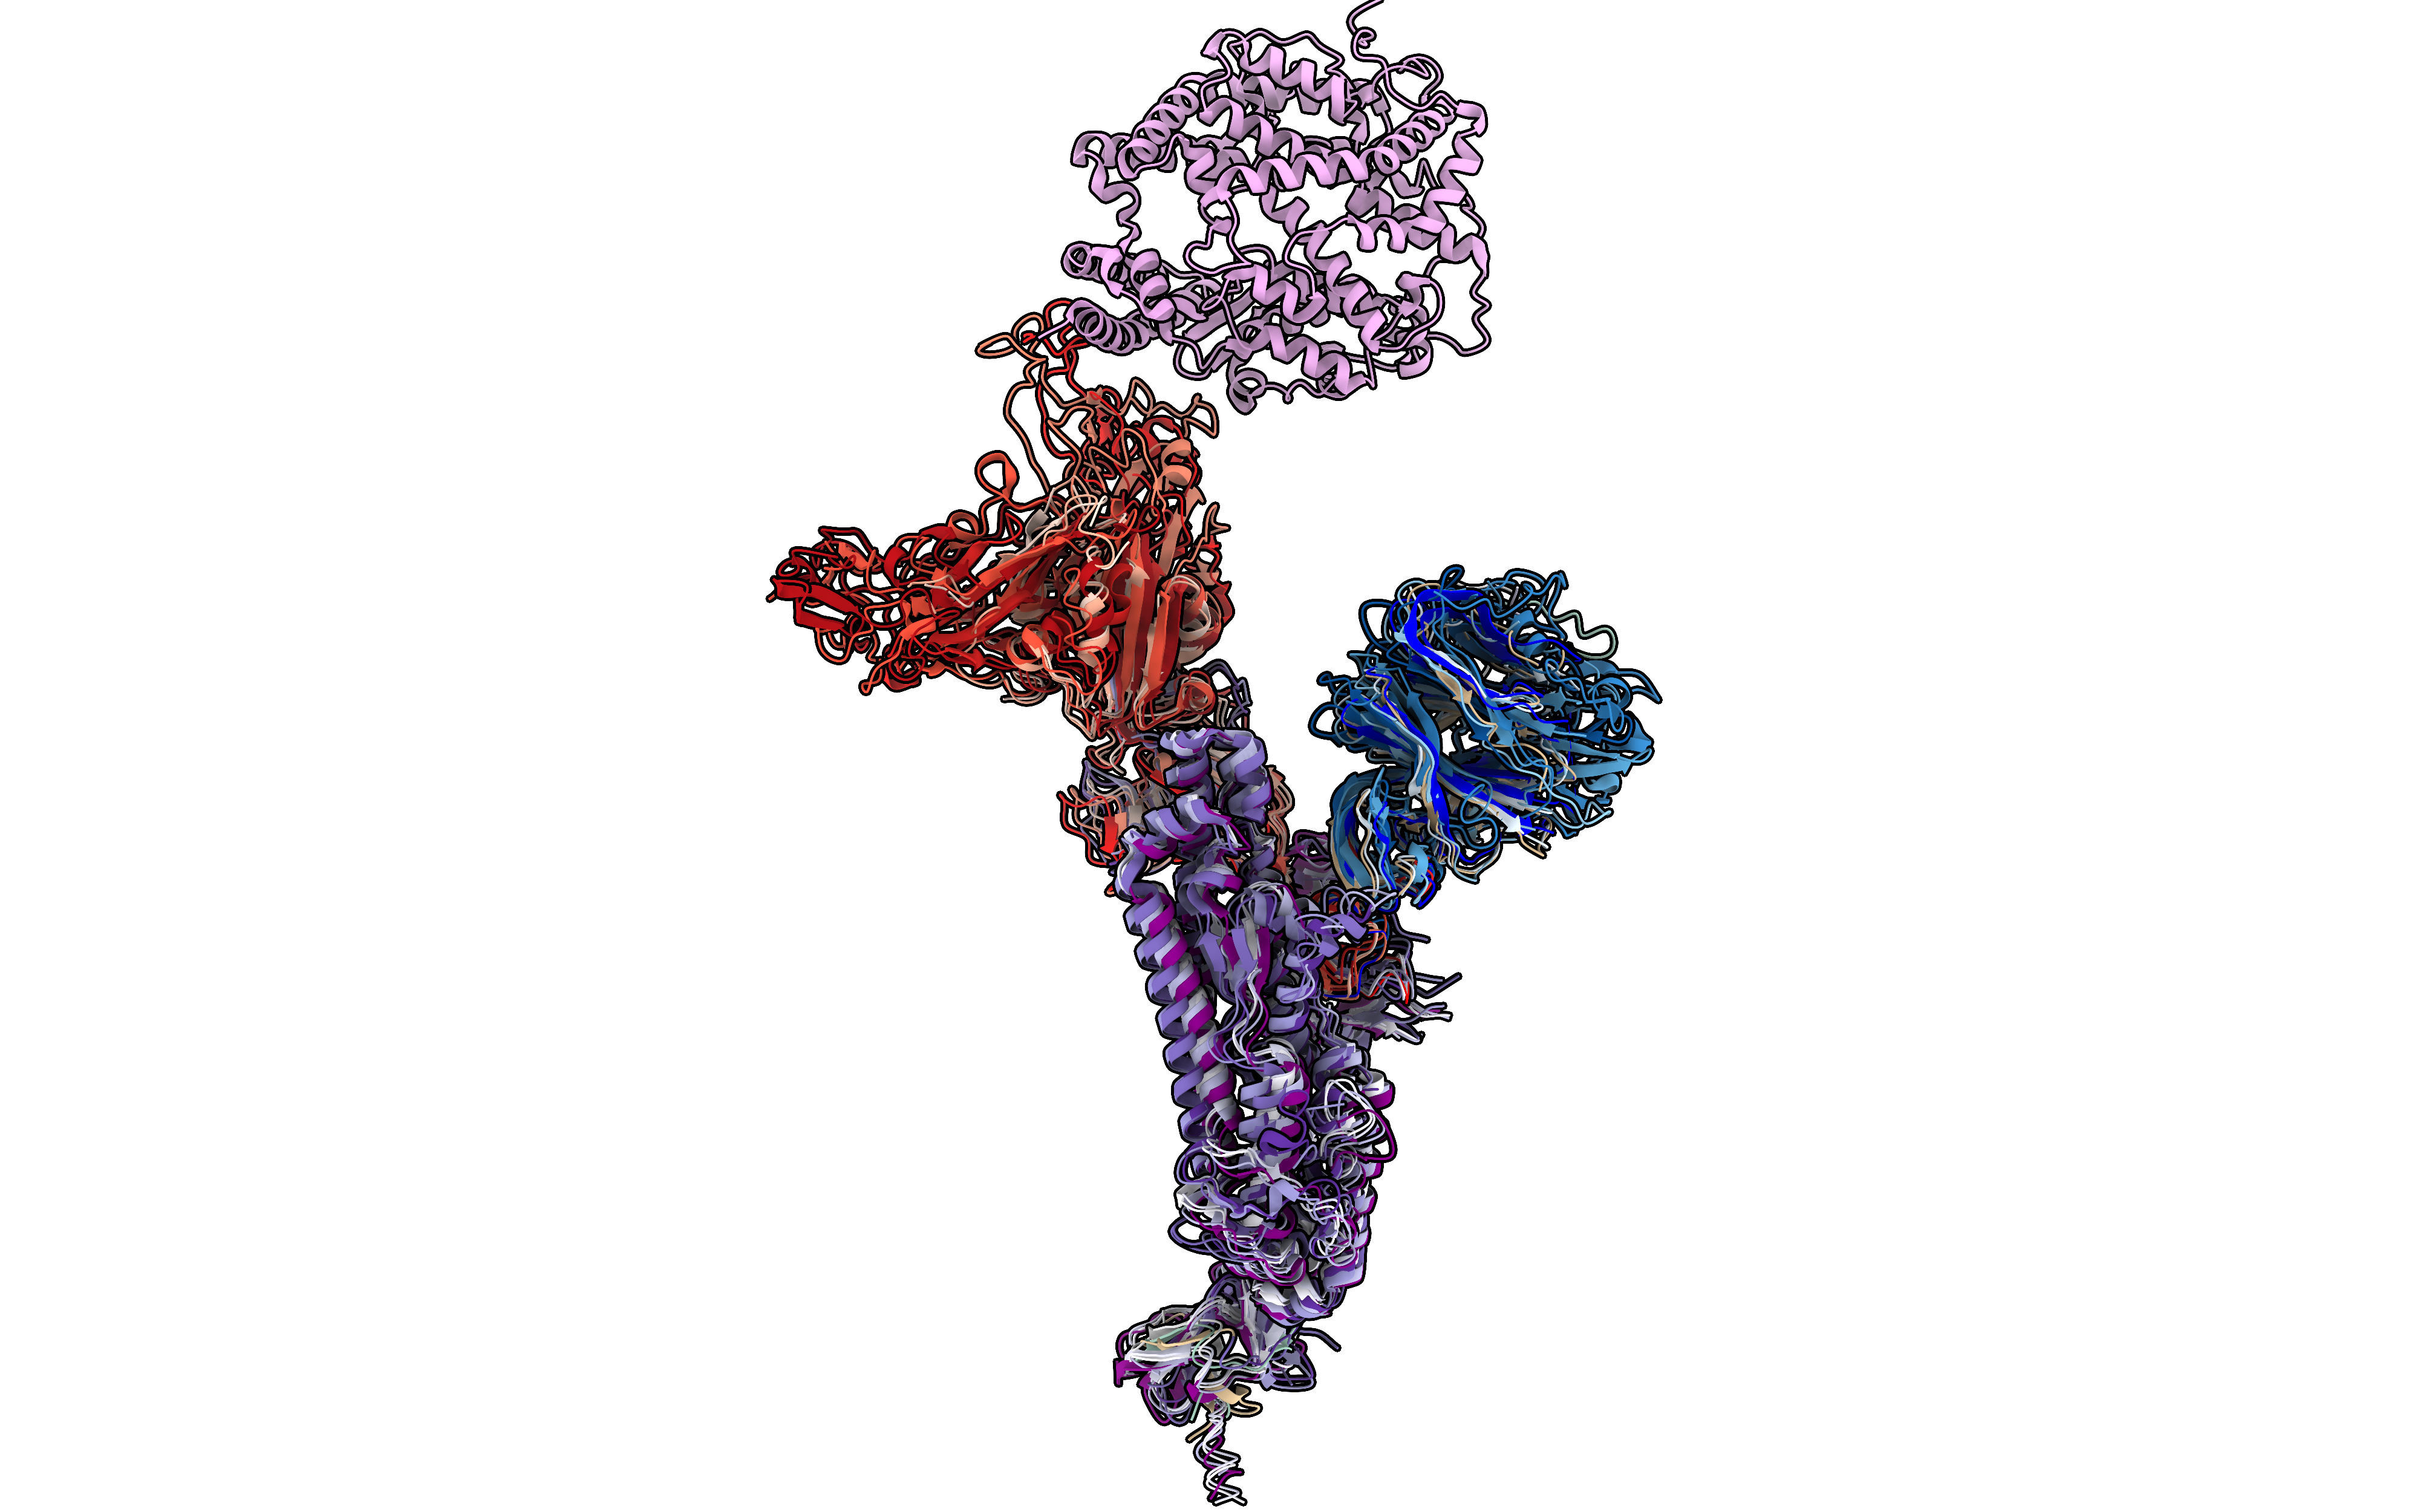
\includegraphics[width=0.85\linewidth]{img/bcov3d_structrures_v3.png}
    \caption{Superposition of six spike protein structures of Betacoronaviruses (\gls{pdb}~\cite{berman2000, rose2010} IDs: 6VXX (SARS-CoV-2, wild type)~\cite{walls2020}, 9CRH (SARS-CoV-2, Delta)~\cite{ke2024}, 8WHS (SARS-CoV-2, Omicron BA.2.86)~\cite{liu2024}, 6NB6 (SARS-CoV)~\cite{walls2019}, 8IFN (MERS-CoV)~\cite{tian2024}, 9BSW (HCoV-HKU1)~\cite{jin2025}, 7SB3 (HCoV-OC43)~\cite{bangaru2022}, 9K75 (BANAL-103)~\cite{li2025}). The spike protein contains two major subunits. The first subunit, S1, typically comprises the \gls{rbd} in the C-terminal (red) and N-terminal (blue) domains. The \gls{rbd} typically attaches to ligands, such as \gls{ace2} (pink) via the receptor-binding motif (RBM). The second subunit, S2 (purple), is typically more conserved and comprises various helical structures, such as the heptad repeat regions HR1 and HR2. Visualization rendered using ChimeraX~\cite{meng2023}.}
    \label{fig:bcov_spike}
\end{figure}